\documentclass[11pt]{report}

\usepackage{iftex}
\ifPDFTeX
  \errmessage{Please compile with XeLaTeX or LuaLaTeX}
\fi

\usepackage{fontspec}
\usepackage{geometry}
\usepackage{xcolor}
\usepackage{microtype}
\usepackage{hyperref}
\usepackage{fancyhdr}
\usepackage{titlesec}
\usepackage[most]{tcolorbox}
\usepackage{amsmath,amssymb,amsthm,mathtools,bm}
\usepackage{enumitem}
\usepackage{booktabs}
\usepackage{etoolbox}
\usepackage[nameinlink,noabbrev]{cleveref}
\usepackage{graphicx} % 使用 \includegraphics
\usepackage{float}    % 使用 [H]
\geometry{
  paperwidth=7.25in,
  paperheight=10in,
  left=0.82in,
  right=0.82in,
  top=0.82in,
  bottom=0.82in,
  headheight=16pt,
  headsep=0.33in,
  footskip=0.42in
}

\IfFontExistsTF{Times New Roman}{\setmainfont{Times New Roman}}{\setmainfont{DejaVu Serif}}
\IfFontExistsTF{Helvetica Neue}{\setsansfont{Helvetica Neue}}{\setsansfont{DejaVu Sans}}
\IfFontExistsTF{JetBrains Mono}{\setmonofont{JetBrains Mono}}{\setmonofont{DejaVu Sans Mono}}

\linespread{1.18}
\setlength{\parindent}{1.4em}
\setlength{\parskip}{0.16em}

% =========================================================
% Colors
% =========================================================
\definecolor{ink}{HTML}{1A1A1A}
\definecolor{muted}{HTML}{5E5E5E}

\definecolor{defBlueBg}{HTML}{EEF7FF}
\definecolor{defBlueD}{HTML}{2C7FB8}

\definecolor{exampleGreenBg}{HTML}{EEF8F0}
\definecolor{exampleGreenD}{HTML}{2E8B57}

\definecolor{theoremPurpleBg}{HTML}{F4EEFF}
\definecolor{theoremProofBg}{HTML}{FFF9FF}
\definecolor{theoremPurpleD}{HTML}{7E57C2}

\definecolor{insightBrownBg}{HTML}{F8EFE6}
\definecolor{insightBrownD}{HTML}{A05A2C}

\definecolor{remarkOrangeBg}{HTML}{FFF4E8}
\definecolor{remarkOrangeD}{HTML}{C06A21}

\hypersetup{
  colorlinks=true,
  linkcolor=defBlueD,
  citecolor=defBlueD,
  urlcolor=defBlueD,
  pdfauthor={MIStatlE},
  pdftitle={Information Theory Lecture Template}
}

% =========================================================
% Chapter title
% =========================================================
% \titleformat{\chapter}[hang]
%   {\normalfont\Huge\bfseries\sffamily\color{ink}}
%   {Chapter \thechapter:}{0.55em}{}
\titleformat{\chapter}[display]
  {\normalfont\Huge\bfseries\sffamily\color{ink}}
  {\Large Chapter \thechapter:}
  {0.35em}
  {}
\titlespacing*{\chapter}{0pt}{0.25em}{1.15em}

% =========================================================
% Header / footer
% Left header: fixed text for all chapters.
% Right header: automatically follows the current chapter title.
% Footer: automatic page number only.
% =========================================================
\renewcommand{\chaptermark}[1]{\markboth{Chapter \thechapter: #1}{}}

\fancyhf{}
\renewcommand{\headrulewidth}{0.35pt}
\renewcommand{\footrulewidth}{0pt}
\fancyhead[L]{\small\sffamily\color{ink}Information Theory}
\fancyhead[R]{\small\sffamily\color{ink}\nouppercase{\leftmark}}
\fancyfoot[C]{\small\thepage}
\pagestyle{fancy}
\fancypagestyle{plain}{%
  \fancyhf{}%
  \renewcommand{\headrulewidth}{0.35pt}%
  \renewcommand{\footrulewidth}{0pt}%
  \fancyhead[L]{\small\sffamily\color{ink}Information Theory}%
  \fancyhead[R]{\small\sffamily\color{ink}\nouppercase{\leftmark}}%
  \fancyfoot[C]{\small\thepage}%
}

% =========================================================
% Lists
% =========================================================
\setlist[itemize]{leftmargin=1.6em,itemsep=0.34em,topsep=0.35em}
\setlist[enumerate]{leftmargin=1.8em,itemsep=0.34em,topsep=0.35em}

% =========================================================
% Shared block styles
% =========================================================
\tcbset{
  lectureblock/.style 2 args={
    enhanced,
    breakable,
    frame hidden,
    boxrule=0pt,
    borderline west={3pt}{0pt}{#1},
    colback=#2,
    arc=0pt,
    outer arc=0pt,
    left=13pt,
    right=11pt,
    top=8pt,
    bottom=8pt,
    boxsep=0pt,
    before skip=0.9em,
    after skip=0.9em
  },
  theoremblock/.style n args={3}{
    enhanced,
    breakable,
    bicolor,
    frame hidden,
    boxrule=0pt,
    borderline west={3pt}{0pt}{#1},
    colback=#2,
    colbacklower=#3,
    arc=0pt,
    outer arc=0pt,
    left=13pt,
    right=11pt,
    top=8pt,
    bottom=8pt,
    middle=5pt,
    boxsep=0pt,
    segmentation style={draw=none},
    before skip=0.9em,
    after skip=0.9em
  }
}

% =========================================================
% Manual blocks
% =========================================================
\newtcolorbox{ExampleBox}{
  lectureblock={exampleGreenD}{exampleGreenBg},
  before upper={\noindent\textbf{\sffamily\color{exampleGreenD}Example.}\space\ignorespaces}
}

\newtcolorbox{InsightBox}{
  lectureblock={insightBrownD}{insightBrownBg},
  before upper={\noindent\textbf{\sffamily\color{insightBrownD}Insight.}\space\ignorespaces}
}

\newtcolorbox{RoadmapBox}{
  lectureblock={defBlueD}{defBlueBg},
  before upper={\noindent\textbf{\sffamily\color{defBlueD}Roadmap.}\space\ignorespaces}
}

% =========================================================
% Theorem block with integrated proof area
%
% Usage:
%   \begin{theorem}[Theorem title]
%   The theorem statement.
%   \tcblower
%   The proof text.
%   \end{theorem}
%
% Upper part: theoremPurpleBg.
% Lower proof part: theoremProofBg.
% The left rule is continuous because both parts are in the same tcolorbox.
% =========================================================
\newtcolorbox[auto counter]{theorem}[1][]{
  theoremblock={theoremPurpleD}{theoremPurpleBg}{theoremProofBg},
  before upper={%
    \noindent\textbf{\sffamily\color{theoremPurpleD}Theorem~\thetcbcounter%
    \ifstrempty{#1}{}{ (#1)}.}\space\ignorespaces
  },
  before lower={\noindent\textbf{\sffamily\color{theoremPurpleD}Proof.}\space\ignorespaces},
  after lower={\hfill\qedsymbol}
}

\newtcolorbox{corollary}[1][]{
  theoremblock={theoremPurpleD}{theoremPurpleBg}{theoremProofBg},
  before upper={%
    \noindent\textbf{\sffamily\color{theoremPurpleD}Corollary~\thetcbcounter%
    \ifstrempty{#1}{}{ (#1)}.}\space\ignorespaces
  },
  before lower={\noindent\textbf{\sffamily\color{theoremPurpleD}Proof.}\space\ignorespaces},
  after lower={\hfill\qedsymbol}
}

\newtcolorbox{property}[1][]{
  theoremblock={theoremPurpleD}{theoremPurpleBg}{theoremProofBg},
  before upper={%
    \noindent\textbf{\sffamily\color{theoremPurpleD}Property~\thetcbcounter%
    \ifstrempty{#1}{}{ (#1)}.}\space\ignorespaces
  },
  before lower={\noindent\textbf{\sffamily\color{theoremPurpleD}Proof.}\space\ignorespaces},
  after lower={\hfill\qedsymbol}
}

\newtcolorbox[auto counter]{lemma}[1][]{
  theoremblock={theoremPurpleD}{theoremPurpleBg}{theoremProofBg},
  before upper={%
    \noindent\textbf{\sffamily\color{theoremPurpleD}Lemma~\thetcbcounter%
    \ifstrempty{#1}{}{ (#1)}.}\space\ignorespaces
  },
  before lower={\noindent\textbf{\sffamily\color{theoremPurpleD}Proof.}\space\ignorespaces},
  after lower={\hfill\qedsymbol}
}

\newtcolorbox[auto counter]{axiom}[1][]{
  theoremblock={theoremPurpleD}{theoremPurpleBg}{theoremProofBg},
  before upper={%
    \noindent\textbf{\sffamily\color{theoremPurpleD}Axiom~\thetcbcounter%
    \ifstrempty{#1}{}{ (#1)}.}\space\ignorespaces
  }
}
% =========================================================
% Definition / remark environments
% =========================================================
\newtheoremstyle{lecturedefinition}
  {0.3em}{0.3em}{}{}%
  {\bfseries\sffamily\color{defBlueD}}{.}{0.45em}{}

\newtheoremstyle{lectureremark}
  {0.3em}{0.3em}{}{}%
  {\bfseries\sffamily\color{remarkOrangeD}}{.}{0.45em}{}

\theoremstyle{lecturedefinition}
\newtheorem{definition}{Definition}

\theoremstyle{lectureremark}
\newtheorem{remark}{Remark}

\tcolorboxenvironment{definition}{lectureblock={defBlueD}{defBlueBg}}
\tcolorboxenvironment{remark}{lectureblock={remarkOrangeD}{remarkOrangeBg}}

% Math helpers
\DeclareMathOperator{\Var}{Var}
\newcommand{\E}{\mathbb{E}}
\newcommand{\norm}[1]{\left\lVert #1 \right\rVert}


% This is the template of blocks
% 
% Definition:
% \begin{definition}[Information]
% \textbf{Concept} this is the content of definition.
% \end{definition}
% 
% Example:
% \begin{ExampleBox}
% This is the content of examples.
% \end{ExampleBox}
% 
% Axiom:
% \begin{axiom}[axiom content]
% This is one axiom.
% \end{axiom}
% 
% Lemma/Theorem
% \begin{lemma}
% Statement of the lemma/theroem
% \tcblower
% Proof of the lemma/theorem
% \end{lemma}
% 
% 
% \begin{InsightBox}
% This is the content of the insight.
% \end{InsightBox}

\begin{document}
\setcounter{chapter}{1}
\chapter{Self-Information and Properties of Entropy}
\begin{center}
by ZYL
\end{center}
\section{Self-Information}
Suppose someone tells us that the sun rose this morning. This statement is not very informative because it describes an event that was almost certain to occur. In contrast, suppose someone tells us that it snowed in a tropical city. This event is highly unexpected, so the statement carries much more information.

This observation suggests that information should depend inversely on probability:
\begin{equation*}
    \begin{aligned}
        \text{highly probable event}&\rightarrow \text{little information}\\
        \text{unlikely event}&\rightarrow\text{much information}
    \end{aligned}
\end{equation*}
Self-information formalizes this idea.

\begin{definition}[Self-Information]
When the outcome $X=x$ is observed, its \textbf{self-information} is defined as:
\begin{equation*}
    i_X(x)\triangleq-\log p_X(x)=\log\frac{1}{p_X(x)}
\end{equation*}
\end{definition}
Self-information measures the amount of surprise associated with observing the outcome $x$. It can also be interpreted as the amount of uncertainty removed after $x$ is observed.

Because
\begin{equation*}
    i_X(x)=\log\frac{1}{p_X(x)}
\end{equation*}
a smaller probability gives a larger value of self-information. Thus,
\begin{equation*}
    p_X(x_1)<p_X(x_2)\;\Rightarrow \; i_X(x_1)>i_X(x_2)
\end{equation*}
The logarithm is used because \textit{information from independent events should add}. For example, if two independent events occur with probability $p(x)$ and $p(y)$, then
\begin{equation*}
    p_{X,Y}(x,y)=p_X(x)p_Y(y)
\end{equation*}
Therefore,
\begin{equation*}
    \begin{aligned}
        i_{X,Y}(x,y)&=-\log p_{X,Y}(x,y)\\
        &=-\log(p_X(x)p_Y(y))\\
        &=-\log p_X(x)-\log p_Y(y)\\
        &=i_X(x)+i_Y(y)
    \end{aligned}
\end{equation*}
Thus, the information carried by two independent observations is the sum of the information carried by each observation.

\textbf{\textcolor{brown}{Nonnegativity of Self-information.}} Since $0<p_X(x)\le 1$, we have
\begin{equation*}
    \log p_X(x)\le 0
\end{equation*}
Therefore,
\begin{equation}
    i_X(x)\ge 0
\end{equation}

\section{Self-Information vs. Entropy}
We can rewrite the entropy as the expectation of self-information:
\begin{equation}
    H(X)=\mathbb{E}_{X\sim p_X}[i_X(X)]
\end{equation}

\begin{property}
Nonnegativity of entropy:
\begin{equation*}
    H(X)\ge 0
\end{equation*}
\tcblower
Since $H(X)=\mathbb{E}_{X\sim p_X}[i_X(X)]$ and \(i_X(X)\geq 0\) almost surely, we have \(H(X)\geq 0\).
Equality holds if and only if \(X\) is deterministic.
\end{property}

\begin{property}
Suppose $X$ has a finite alphabet $\mathcal{X}$. Then
\begin{equation*}
    H(X)\le \log |\mathcal{X}|
\end{equation*}
Equality holds if and only if $X$ is uniformly distributed:
\begin{equation*}
    p_X(x)=\frac{1}{|\mathcal{X}|},\quad\forall x\in\mathcal{X}
\end{equation*}
\tcblower
We will prove it in the next chapter.
\end{property}

\section{Joint Self-Information \& Joint Entropy}
\begin{definition}[Joint Self-Information \& Joint Entropy]
    Consider two discrete random variables $X$ and $Y$ with joint PMF $p_{X,Y}(x,y)=P(X=x, Y=y)$, then the \textbf{joint self-information} of the outcome $(x,y)$ is
    \begin{equation*}
        i_{X,Y}(x,y)\triangleq-\log p_{X,Y}(x,y)
    \end{equation*}
    The \textbf{joint entropy} if $X$ and $Y$ is defined as:
    \begin{equation*}
        H(X,Y)\triangleq-\sum_{x\in\mathcal{X}}\sum_{y\in\mathcal{Y}}p_{X,Y}(x,y)\log p_{X,Y}(x,y)
    \end{equation*}
\end{definition}
Using $i(x,y)=-\log p_{X,Y}(x,y)$, we obtain
\begin{equation*}
    \begin{aligned}
        H(X,Y)&=-\sum_{x,y}p_{X,Y}(x,y)\log p_{X,Y}(x,y)\\
        &=\sum_{x,y}p_{X,Y}(x,y)i_{X,Y}(x,y)
    \end{aligned}
\end{equation*}
Therefore,
\begin{equation}
    H(X,Y)=\mathbb{E}_{(X,Y)\sim p_{X,Y}}[i(X,Y)]
\end{equation}
This is an equivalent form derived from the definition.

\textbf{\textcolor{brown}{Nonnegativity of joint entropy.}} Because $0<p(x,y)\le 1$, we have $-\log p_{X,Y}(x,y)\ge 0$, then
\begin{equation}
    H(X,Y)\ge 0
\end{equation}

\begin{corollary}
Suppose $X$ and $Y$ are \textit{independent}. Then
\begin{equation*}
    H(X,Y)=H(X)+H(Y)
\end{equation*}
\tcblower
Since $X$ and $Y$ are independent, then
\begin{equation*}
    p_{X,Y}(x,y)=p_X(x)p_Y(y)
\end{equation*}
We obtain
\begin{equation*}
    \begin{aligned}
        H(X,Y)&=-\sum_{x,y}p_{X,Y}(x,y)\log p_{X,Y}(x,y)\\
        &=-\sum_{x,y}p_{X}(x)p_Y(y)\log \left(p_{X}(x)p_Y(y)\right)\\
        &=-\sum_{x,y}p_X(x)p_Y(y)\left[\log p_X(x)+\log p_Y(y) \right]\\
    \end{aligned}
\end{equation*}
Separate the two terms:
\begin{equation*}
    \begin{aligned}
        H(X,Y)&=-\sum_{x,y}p_X(x)p_{Y}(y)\log p_{X}(x)-\sum_{x,y}p_X(x)p_Y(y)\log p_Y(y)\\
        &=-\sum_{x}p_X(x)\log p_{X}(x)-\sum_{y}p_Y(y)\log p_{Y}(y)\\
        &=H(X)+H(Y)\\
    \end{aligned}
\end{equation*}
\end{corollary}
Note that in general, $H(X,Y)\ne H(X)+H(Y)$. The equality holds only under independence.

\section{Conditional Self-Information \& Conditional Entropy}
Before defining conditional information quantities, recall the conditional probability:
\begin{equation*}
    p_{X\mid Y}(x\mid y)\triangleq \frac{p_{X,Y}(x,y)}{p_Y(y)},\quad \text{for }p_Y(y)>0 
\end{equation*}
This is the probability of observing $X=x$ after learning that $Y=y$.

Suppose that $Y=y$ has already been observed. The uncertainty associated with $X=x$ should now be measured using the conditional probability $p_{X\mid Y}(x\mid y)$, rather than the marginal probability $p_X(x)$.

\begin{definition}[Conditional Self-Information]
The conditional self-information is defined as:

\begin{equation*}
    i_{X\mid Y}(x\mid y)\triangleq -\log p_{X\mid Y}(x\mid y)
\end{equation*}
\end{definition}
It measures the remaining surprise of observing $x$ when $y$ is already known.

\begin{ExampleBox}
Let $X$: whether it rains, $Y$: whether a person carries an umbrella. Suppose $P(X=\text{rain})=0.3$, and $P(X=\text{rain}\mid Y=\text{umbrella})=0.8$.

Before observing the umbrella,
\begin{equation*}
    i(\text{rain})=-\log 0.3\approx 1.737\text{ bits}
\end{equation*}
After observing the umbrella,
\begin{equation*}
    i(\text{rain}\mid \text{umbrella})=-\log 0.8\approx 0.322\text{ bits}
\end{equation*}
Seeing an umbrella makes rain less surprising because the conditional probability of rain becomes larger.
\end{ExampleBox}

For a particular observed value $Y=y$, the remaining uncertainty of $X$ is the entropy of the conditional distribution $p_{X\mid Y}(x\mid y)$.
\begin{definition}[Conditional Entropy]
The conditional entropy is defined as:
\begin{equation*}
    H(X\mid Y)\triangleq \mathbb{E}_{Y}[H(X\mid Y=y)]=-\sum_{x\in \mathcal{X}}\sum_{y\in \mathcal{Y}}p_{X,Y}(x,y)\log p(x\mid y)
\end{equation*}
\end{definition}
The following provides a derivation of this definition. When $Y=y$ is given,
\begin{equation*}
    \begin{aligned}
        H(X\mid Y=y)&=\mathbb{E}_{X\mid y}\left[i(X\mid Y=y)\right]\\
        &=-\sum_{x\in\mathcal{X}}p(x\mid y)\log p_{X\mid Y}(x\mid y)\\
    \end{aligned}
\end{equation*}
Then,
\begin{equation*}
    \begin{aligned}
        H(X\mid Y)&\triangleq\mathbb{E}_{Y}[H(X\mid Y=y)]\\
        &=\sum_{y\in \mathcal{Y}}p_Y(y)H(X\mid Y=y)\\
        &=-\sum_{y\in\mathcal{Y}}p_Y(y)\sum_{x\in\mathcal{X}}p_{X\mid Y}(x\mid y)\log p_{X\mid Y}(x\mid y)\\
        &=-\sum_{x\in\mathcal{X}}\sum_{y\in\mathcal{Y}}p_{X,Y}(x,y)\log p_{X\mid Y}(x\mid y)
    \end{aligned}
\end{equation*}
Therefore, there is a derived equivalent form of conditional entropy:
\begin{equation}
    H(X\mid Y)=\mathbb{E}_{(X,Y)\sim p_{X,Y}}\left[i(X\mid Y)\right]
\end{equation}
It measures the \textit{average uncertainty of $X$ over all $y$.}

\begin{ExampleBox}
Let $X$ be uniformly distributed over $\{0,1,2,3\}$, and define Y by:
\begin{equation*}
    Y=\begin{cases}
        0,& X\in\{0,1\}\\
        1,& X\in\{2,3\}
    \end{cases}
\end{equation*}
Then 
\begin{equation*}
P(Y=0)=P(Y=1)=\frac{1}{2}
\end{equation*}
and
\begin{equation*}
    \begin{aligned}
        H(X\mid Y=0)=&-p(X=0\mid Y=0)\log p(X=0\mid Y=0)\\
        &-p(X=1\mid Y=0)\log p(X=1\mid Y=0)\\
        =&-\frac{1}{2}\log\frac{1}{2}-\frac{1}{2}\log \frac{1}{2}\\
        =&1\text{ bit}\\
        H(X\mid Y=1)=&-p(X=2\mid Y=1)\log p(X=2\mid Y=1)\\
        &-p(X=3\mid Y=1)\log p(X=3\mid Y=1)\\
        =&-\frac{1}{2}\log\frac{1}{2}-\frac{1}{2}\log \frac{1}{2}\\
        =&1\text{ bit}\\
    \end{aligned}
\end{equation*}
So the conditional entropy is
\begin{equation*}
    \begin{aligned}
        H(X\mid Y)&=p(Y=0)H(X\mid Y=0)+p(Y=1)H(X\mid Y=1)\\
        &=\frac{1}{2}\cdot 1+\frac{1}{2}\cdot 1\\
        &= 1\text{ bit}
    \end{aligned}
\end{equation*}
Also, we compute that $H(X)=2\text{ bits}$, which implies that observing $Y$ removes one of the original two bits of uncertainty.
\end{ExampleBox}
\section{Properties of Conditional Entropy}
\begin{property}
\newline
1. Nonnegativity of conditional entropy
\begin{equation*}
    H(X\mid Y)\ge 0
\end{equation*}
2. Conditioning a variable on itself
\begin{equation*}
    H(X\mid X)=0
\end{equation*}
3. If $X$ and $Y$ are \textit{independent}, then
\begin{equation*}
    H(X\mid Y)=H(X)
\end{equation*}
4. For discrete random variables $X$ and $Y$,
\begin{equation*}
    H(X\mid Y)\le H(X)
\end{equation*}
Equality holds if and only if $X$ and $Y$ are independent.
\tcblower
\newline
1. Because $0<p_{X\mid Y}(x\mid y)\le 1$, we have $i_{X\mid Y}(x\mid y)=-\log p_{X\mid Y}(x\mid y)\ge 0$. Since $H(X\mid Y)=\mathbb{E}[i(X\mid Y)]$, then $H(X\mid Y)\ge 0$.

2. Once $X$ is known, its value is certain. For every outcome $x$ with positive probability,
\begin{equation*}
    p(X=x\mid X=x)=1
\end{equation*}
Hence, $i(x\mid x)=-\log 1=0$. Taking the expectation, $H(X\mid X)=0$.

3. If $X$ and $Y$ are independent, we have:
\begin{equation*}
    p_{X\mid Y}(x\mid y)=p_X(x)\Rightarrow p_{X,Y}(x,y)=p_X(x)p_Y(y)
\end{equation*}
Then,
\begin{equation*}
    \begin{aligned}
        H(X\mid Y)&=-\sum_{x\in\mathcal{X}}\sum_{y\in\mathcal{Y}}p_{X,Y}(x,y)\log p_{X\mid Y}(x\mid y)\\
        &=-\sum_{x\in\mathcal{X}}\sum_{y\in\mathcal{Y}}p_X(x)p_Y(y)\log p_X(x) \\
        &=-\sum_{y\in\mathcal{Y}}p_Y(y)\sum_{x\in\mathcal{X}}p_X(x)\log p_X(x)\\
        &=-\sum_{x\in\mathcal{X}}p_X(x)\log p_X(x)\\
        &=H(X)
    \end{aligned}
\end{equation*}
4. We know that $\ln t \le t-1,\forall t>0$. Dividing both sides by $\ln 2$ gives
\begin{equation*}
    \log t\le\frac{t-1}{\ln 2}
\end{equation*}
Taking the difference between $H(X)$ and $H(X\mid Y)$, we get
\begin{equation*}
\begin{aligned}
    H(X)-H(X\mid Y)=&-\sum_{x\in \mathcal{X}}p_X(x)\log p_X(x)+\sum_{x\in\mathcal{X}}\sum_{y\in\mathcal{Y}}p_{X,Y}(x,y)\log p_{X\mid Y}(x\mid y)\\
    =&-\sum_{x\in \mathcal{X}}\sum_{y\in\mathcal{Y}}p_{X,Y}(x,y)\log p_X(x)\\
    &+\sum_{x\in\mathcal{X}}\sum_{y\in\mathcal{Y}}p_{X,Y}(x,y)\log p_{X\mid Y}(x\mid y)\\
    =& \sum_{x\in\mathcal{X}}\sum_{y\in\mathcal{Y}}p_{X,Y}(x,y)\log\frac{p_{X\mid Y}(x\mid y)}{p_X(x)}\\
    =&-\sum_{x\in\mathcal{X}}\sum_{y\in\mathcal{Y}}p_{X,Y}(x,y)\log\frac{p_X(x)p_Y(y)}{p_{X, Y}(x, y)}\\
\end{aligned}
\end{equation*}
Applying the inequality, we get
\begin{equation*}
\begin{aligned}
    H(X)-H(X\mid Y)\ge&-\frac{1}{\ln 2}\sum_{x\in\mathcal{X}}\sum_{y\in\mathcal{Y}}p_{X,Y}(x,y)\left(\frac{p_X(x)p_Y(y)}{p_{X, Y}(x, y)}-1\right)\\
    =&-\frac{1}{\ln 2}\left(\sum_{x\in\mathcal{X}}\sum_{y\in\mathcal{Y}}p_X(x)p_Y(y)-\sum_{x\in\mathcal{X}}\sum_{y\in\mathcal{Y}}p_{X,Y}(x,y)\right)\\
    =&-\frac{1}{\ln 2}\cdot (1-1)\\
    =&0
\end{aligned}
\end{equation*}
Therefore, $H(X)\ge H(X\mid Y)$. Equality holds when \begin{equation*}
    \log\frac{p_X(x)p_Y(y)}{p_{X,Y}(x,y)}=\frac{1}{\ln 2}\left(\frac{p_X(x)p_Y(y)}{p_{X,Y}(x,y)}-1\right)
\end{equation*}
that is
\begin{equation*}
\frac{p_X(x)p_Y(y)}{p_{X,Y}(x,y)}=1\Rightarrow p_X(x)p_Y(y)=p_{X,Y}(x,y)
\end{equation*}
which means $X$ and $Y$ are independent.
\end{property}

\section{Chain Rule for Entropy}
\begin{theorem}
Chain Rule:
\begin{equation*}
\begin{aligned}
    H(X,Y)&=H(Y)+H(X\mid Y)\\
    H(X,Y)&=H(X)+H(Y\mid X)
\end{aligned}
\end{equation*}
\tcblower
\begin{equation*}
\begin{aligned}
H(X\mid Y)\triangleq& \mathbb{E}_{X,Y}\left[i(X\mid Y)\right]\\
=&-\sum_{x\in\mathcal{X}}\sum_{y\in\mathcal{Y}}p_{X,Y}(x,y)\log p_{X\mid Y}(x\mid y)\\
=& -\sum_{x\in\mathcal{X}}\sum_{y\in\mathcal{Y}}p_{X,Y}(x,y)\log \frac{p_{X,Y}(x,y)}{p_Y(y)}\\
=&\sum_{x\in\mathcal{X}}\sum_{y\in\mathcal{Y}}p_{X,Y}(x,y)\log p_Y(y)-\sum_{x\in\mathcal{X}}\sum_{y\in\mathcal{Y}}p_{X,Y}(x,y)\log p_{X,Y}(x,y)\\
=&\sum_{y\in\mathcal{Y}}p_Y(y)\log p_Y(y)+H(X,Y)\\
=&-H(Y)+H(X,Y)
\end{aligned}
\end{equation*}
Rearranging gives $H(X,Y)=H(Y)+H(X\mid Y)$.
\end{theorem}
The factorization $p_{X,Y}(x,y)=p_Y(y)p_{X\mid Y}(x\mid y)$ suggests a two-stage description of the pair $(X,Y)$: 1. first describe $Y$, 2. then describe $X$ after $Y$ is known. The average information required in the first stage is $H(Y)$, and the average additional information required in the second stage is $H(X\mid Y)$.

Let $X^n=(X_1, X_2,\cdots, X_n)$, we can write the generalized chain rule as:
\begin{equation}
    H(X^n)=\sum_{i=1}^nH(X_i\mid X^{i-1})
\end{equation}
For three variables, we have
\begin{equation*}
    H(X_1, X_2, X_3)=H(X_1)+H(X_2\mid X_1)+H(X_3\mid X_1, X_2)
\end{equation*}

\section{Mutual Information}
Before observing $Y$, the uncertainty of $X$ is $H(X)$. After observing $Y$, the remaining uncertainty is $H(X\mid Y)$. The difference measures the average reduction in uncertainty about $X$ produced by observing $Y$.
\begin{definition}[Self Mutual Information]
The definition of \textbf{self mutual information} is
\begin{equation*}
    i_{X;Y}(x;y)\triangleq i_X(x)-i_{X\mid Y}(x\mid y)
\end{equation*}
\end{definition}
Intuitively, $i_{X;Y}(x;y)$ measures the change in the self-information of \(x\) after \(y\) is observed.

Substituting $i_X(x)=-\log p_X(x)$ and $i_{X\mid Y}(x\mid y)=-\log p_{X\mid Y}(x\mid y)$, we derive
\begin{equation*}
    i_{X;Y}(x;y)=-\log p_X(x)+\log p_{X\mid Y}(x\mid y)
    =\log \frac{p_{X,Y}(x,y)}{p_X(x)p_Y(y)}
\end{equation*}
This form compares the actual joint probability with the joint probability expected under independence. The product $p_X(x)p_Y(y)$ is the joint probability that would occur if $X$ and $Y$ were independent. Therefore, $i_{X;Y}(x;y)>0$ means that $x$ and $y$ occur together more often than independence predicts, $i_{X;Y}(x;y)=0$ means that the pair behaves as expected under independence, and $i_{X;Y}(x;y)<0$ means that the pair occurs less often than independence predicts. 

\textbf{\textcolor{brown}{Symmetry of self mutual information.}} For the derived form, we find that the expression is unchanged if $x$ and $y$ are exchanged. Therefore,
\begin{equation}
    i_{X;Y}(x;y)=i_{Y;X}(y;x)
\end{equation}
\begin{ExampleBox}
Suppose $P(\text{rain})=0.2$, $P(\text{umbrella})=0.3$, and $P(\text{rain}, \text{umbrella})=0.18$. Using the derived probability-ratio form,
\begin{equation*}
    i(\text{rain};\text{umbrella})=\log\frac{0.18}{0.2\times 0.3}\approx1.585\text{ bits}
\end{equation*}
The positive value means that rain and umbrella use occur together more frequently than independence would predict.
\end{ExampleBox}

\begin{definition}[Mutual Information]
Mutual information is the expected self mutual information:
\begin{equation*}
    I(X;Y)\triangleq \mathbb{E}_{(X,Y)\sim p_{X,Y}}[i(X;Y)]
\end{equation*}
\end{definition}
Expanding the expectation gives
\begin{equation*}
    I(X;Y)=\sum_{x\in\mathcal{X}}\sum_{y\in\mathcal{Y}}p_{X,Y}(x,y)i_{X;Y}(x;y)=\sum_{x\in\mathcal{X}}\sum_{y\in\mathcal{Y}}p_{X,Y}(x,y)\log\frac{p_{X,Y}(x,y)}{p_X(x)p_Y(y)}
\end{equation*}
Since
\begin{equation*}
\begin{aligned}
    I(X;Y)\triangleq& \mathbb{E}_{(X,Y)\sim p_{X,Y}}[i_{X;Y}(X;Y)]\\
    =& \mathbb{E}_{(X,Y)\sim p_{X,Y}}[i_X(X)-i_{X\mid Y}(X\mid Y)]\\
    =& \mathbb{E}_{(X,Y)\sim p_{X,Y}}[i_X(X)]-\mathbb{E}_{(X,Y)\sim p_{X,Y}}[i_{X\mid Y}(X\mid Y)]\\
    =&\mathbb{E}_{X\sim p_X}[i_X(X)]-\mathbb{E}_{(X,Y)\sim p_{X,Y}}[i_{X\mid Y}(X\mid Y)]\\
    =& H(X)-H(X\mid Y)
\end{aligned}
\end{equation*}

Therefore, we obtain
\begin{equation}
    I(X;Y)=H(X)-H(X\mid Y)
\end{equation}

Mutual information measures how much knowledge of one random variable reduces uncertainty about the other. Before observing $Y$, the uncertainty about $X$ is $H(X)$. After observing $Y$, the remaining uncertainty is $H(X\mid Y)$. The difference between these quantities is the information that $Y$ provides about $X$.

Therefore, large $I(X;Y)$ means that observing one rv strongly reduces uncertainty about the other. Small $I(X;Y)$ means that one rv provides little information about the other. $I(X;Y)=0$ means that $X$ and $Y$ are independent. And we have
\begin{equation}
    I(X;Y)=0 \quad\Longleftrightarrow\quad X \text{ and }Y \text{ are independent}
\end{equation}
Mutual information measures general statistical dependence.

Substituting $H(X\mid Y)=H(X,Y) - H(Y)$, we get
\begin{equation*}
\begin{aligned}
    I(X;Y)=&H(X)-H(X\mid Y)\\
    =&H(X)-(H(X,Y)-H(Y))\\
    =& H(X)+H(Y)-H(X,Y)
\end{aligned}
\end{equation*}
\begin{property}
\newline
1. Nonnegativity:
\begin{equation*}
    I(X;Y)\ge 0
\end{equation*}
2. Symmetry:
\begin{equation*}
    I(X;Y)=I(Y;X)
\end{equation*}
3. Upper bound
\begin{equation*}
    I(X;Y)\le \min\left\{H(X), H(Y)\right\}
\end{equation*}
4. Mutual information is the measure of independence:
\begin{equation*}
    I(X;Y)=0\quad \Longleftrightarrow \quad X\text{ and } Y\text{ are independent}
\end{equation*}
\tcblower
\newline
1. 
\begin{equation*}
    \begin{aligned}
        I(X;Y)\triangleq& \mathbb{E}_{(X,Y)\sim p_{X,Y}}[i(X;Y)] \\
        =&\sum_{x\in\mathcal{X}}\sum_{y\in\mathcal{Y}}p_{X,Y}(x,y)\log\frac{p_{X,Y}(x,y)}{p_X(x)p_Y(y)}\\
        =&-\frac{1}{\ln2}\sum_{x\in\mathcal{X}}\sum_{y\in\mathcal{Y}}p_{X,Y}(x,y)\ln\frac{p_X(x)p_Y(y)}{p_{X,Y}(x,y)}\\
        \ge &-\frac{1}{\ln2}\sum_{x\in\mathcal{X}}\sum_{y\in\mathcal{Y}}p_{X,Y}(x,y)\left(\frac{p_X(x)p_Y(y)}{p_{X,Y}(x,y)}-1\right)\\
        =&-\frac{1}{\ln2}\sum_{x\in\mathcal{X}}\sum_{y\in\mathcal{Y}}(p_X(x)p_Y(y)-p_{X,Y}(x,y))\\
        =&-\frac{1}{\ln2}(1-1)\\
        =&0
    \end{aligned}
\end{equation*}
2. Since exchanging $X$ and $Y$ gives identical expressions, we obtain $I(X;Y)=I(Y;X)$.

3. Using $I(X;Y)=H(X)-H(X\mid Y)$ and $H(X\mid Y)\ge 0$, we obtain $I(X;Y)\le H(X)$. Similarly, $I(X;Y)\le H(Y)$. Therefore,
\begin{equation*}
    I(X;Y)\le \min\{H(X),H(Y)\}
\end{equation*}
4. The property has been proved above.
\end{property}

We can draw a Venn diagram to show the relationship among entropy $H(X), H(Y)$, conditional entropy $H(X\mid Y), H(Y\mid X)$, and mutual information $I(X;Y)$ as follows:
\begin{figure}[H]
    \centering
    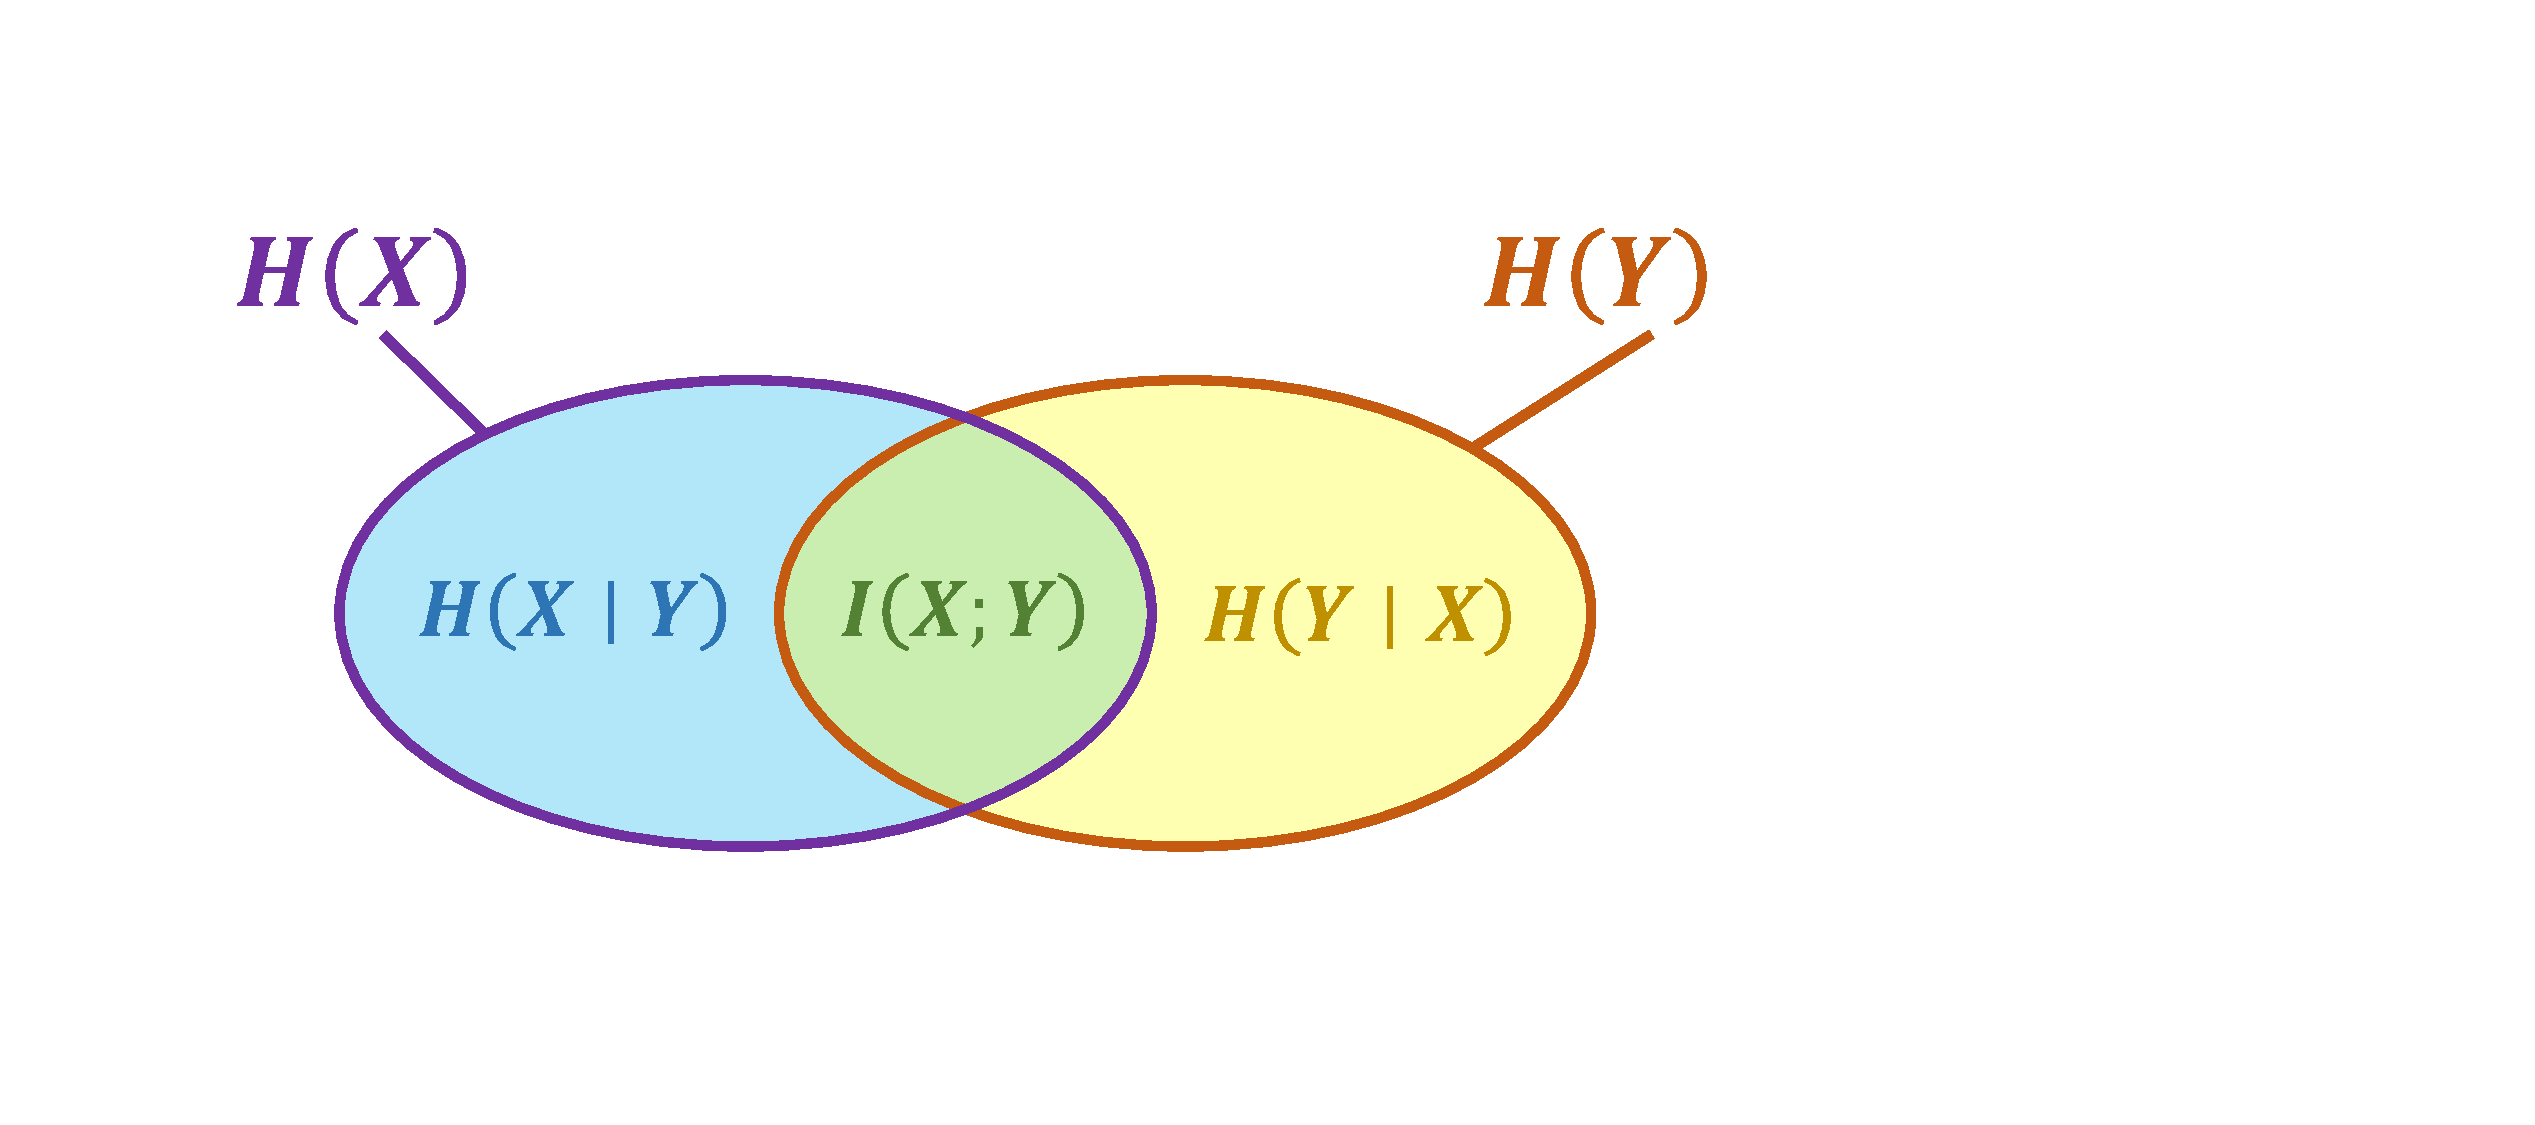
\includegraphics[width=0.5\linewidth]{figure.pdf}
\label{fig:relationship_between_entropy_and_mutual_information}
\end{figure}

\noindent\textbf{\textit{Exercise}}
\vspace{3pt}
\hrule
\vspace{6pt}
\noindent 1. (\textit{Information cannot increase under deterministic processing.}) Let $X$ and \(Y\) be discrete random variables, and let $Z=g(Y)$ for some deterministic function $g$. Prove that
\begin{equation*}
    I(X;Z)\le I(X;Y).
\end{equation*}

\noindent 2. Let $X$, $Y$, $Z$ be discrete random variables. Prove that
\begin{equation*}
    H(X,Y)+H(Y,Z)\ge H(Y)+H(X,Y,Z)
\end{equation*}

\noindent 3. Let $X_1,\dots, X_n$ be discrete random variables. Using the general chain rule, prove that
\begin{equation*}
H(X_1,\cdots, X_n)\le \sum_{i=1}^n H(X_i)
\end{equation*}
and that equality holds if and only if $X_1,\dots, X_n$ are mutually independent.

\noindent 4. (\textit{Han's Inequality}) Let $X_1, \dots, X_n$ be discrete random variables, and let
$X_{-i}=(X_1,\dots,\allowbreak X_{i-1},X_{i+1},\dots,X_n)$ denote the collection obtained by removing $X_i$. Prove that
\begin{equation*}
    (n-1)H(X_1,\dots, X_n)\le \sum_{i=1}^n H(X_{-i})
\end{equation*}

\noindent 5. (\textit{Concavity of entropy}) Let $p$ and $q$ be two PMFs on the same finite alphabet $\mathcal{X}$, and let $r(x)=\lambda p(x)+(1-\lambda)q(x),0<\lambda<1$.
Show that
\begin{equation*}
    H(r)\ge \lambda H(p)+(1-\lambda)H(q)
\end{equation*}
and that equality holds if and only if $p(x)=q(x)$ for every $x\in\mathcal{X}$.

\noindent 6. Let $T=g(Y)$ be a deterministic function of $Y$. Assume that for every $y$ with $p_Y(y)>0$, $p_{X\mid Y}(x\mid y)=p_{X\mid T}(x\mid g(y))$ for all $x$. Prove that
\begin{equation}
    I(X;T)=I(X;Y).
\end{equation}
\end{document}
